% ======================================================================
% fig_pipeline -- standalone build of a figure that main.tex also draws inline.
% ----------------------------------------------------------------------
% The tikzpicture below is copied VERBATIM from main.tex, so this file and
% the inline version render identically. Build with:
%     pdflatex fig_pipeline.tex
% The standalone class crops the PDF to the picture's bounding box, so no
% trim/clip is ever needed in the paper.
%
% Fonts: the picture inherits times/helvet, so every glyph is Type 1 and
% embedded by pdflatex. Nothing is rasterised, so DPI does not apply.
% ======================================================================
\documentclass[border=2pt]{standalone}

\usepackage{times}
\usepackage{helvet}
\usepackage{courier}
\usepackage{amsmath}
\usepackage{amssymb}
\usepackage{xcolor}
\usepackage{pifont}
\usepackage{tikz}
\usetikzlibrary{arrows.meta,positioning}

%% ======================================================================
%% preamble-figures.tex
%% ----------------------------------------------------------------------
%% Every definition the figures need, kept identical to main.tex's preamble.
%% Shared by the standalone builds in this folder; main.tex carries its own
%% copy so that the submitted source stays a single .tex file.
%% ======================================================================

\providecommand{\method}{\textsc{ESV}}

%% --- comparison-table glyphs (fig_trap uses \yes / \no) ---------------
\definecolor{okgreen}{RGB}{0,122,87}
\definecolor{okred}{RGB}{176,42,32}
\providecommand{\yes}{\textcolor{okgreen}{\ding{51}}}
\providecommand{\no}{\textcolor{okred}{\ding{55}}}
\providecommand{\na}{\textcolor{black!45}{--}}

%% --- figure fills, shaded by what each step costs ---------------------
\definecolor{cshared}{RGB}{226,226,226}
\definecolor{ccode}{RGB}{205,228,243}
\definecolor{ccall}{RGB}{252,230,192}
\definecolor{ccallb}{RGB}{191,118,0}
\definecolor{cout}{RGB}{206,238,227}
\definecolor{ctrap}{RGB}{250,222,218}

%% --- plot colours and markers -----------------------------------------
%% Marker shapes are core TikZ nodes, so every glyph is vector and uses the
%% document's Type 1 text fonts: no Type 3 subsets, no raster, nothing to crop.
\definecolor{pblue}{RGB}{31,97,160}
\definecolor{pgreen}{RGB}{0,122,87}
\definecolor{pgrey}{RGB}{95,95,95}
\providecommand{\mkopensq}[2]{\node[draw=#2,fill=white,line width=.6pt,rectangle,inner sep=1.5pt] at #1 {};}
\providecommand{\mkfillsq}[2]{\node[draw=#2,fill=#2,rectangle,inner sep=1.5pt] at #1 {};}
\providecommand{\mkopenci}[2]{\node[draw=#2,fill=white,line width=.6pt,circle,inner sep=1.5pt] at #1 {};}
\providecommand{\mkfillci}[2]{\node[draw=#2,fill=#2,circle,inner sep=1.5pt] at #1 {};}
%% #1 x, #2 centre, #3 half-width of the interval, #4 colour (needs x=1cm)
\providecommand{\ebar}[4]{%
  \draw[#4,line width=.5pt] (#1,{#2-#3}) -- (#1,{#2+#3});
  \draw[#4,line width=.5pt] ({#1-0.055},{#2-#3}) -- ({#1+0.055},{#2-#3});
  \draw[#4,line width=.5pt] ({#1-0.055},{#2+#3}) -- ({#1+0.055},{#2+#3});}

%% --- \cost is used inside the three schematic figures -----------------
\providecommand{\cost}{\scriptsize}


\begin{document}
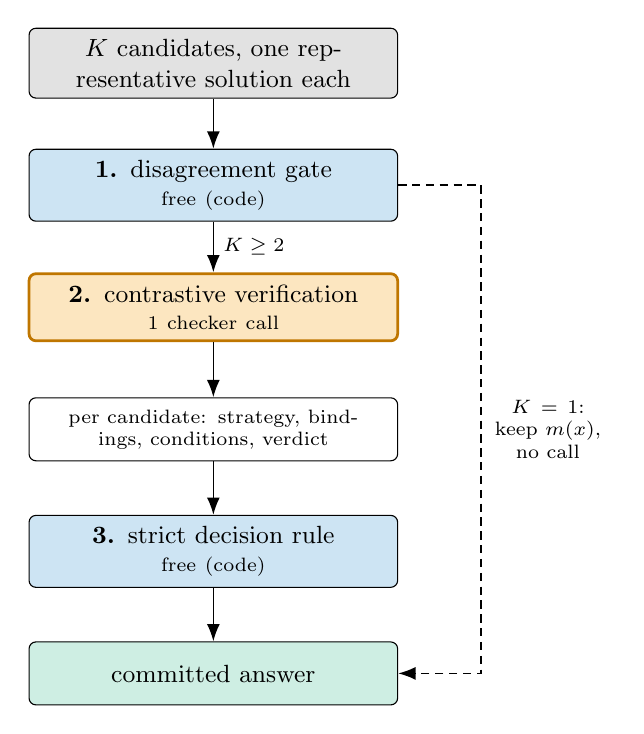
\begin{tikzpicture}[
  font=\small,
  base/.style={draw, rounded corners=2.5pt, align=center, inner sep=4pt,
               text width=44mm, minimum height=8mm},
  shared/.style={base, fill=cshared},
  code/.style={base, fill=ccode},
  call/.style={base, fill=ccall, draw=ccallb, line width=1pt},
  outbox/.style={base, fill=cout},
  fields/.style={base, fill=white, font=\scriptsize},
  ar/.style={-{Latex[length=2.2mm]}, semithick},
  cost/.style={font=\scriptsize},
  side/.style={font=\scriptsize, align=center, text width=15mm},
]
\node[shared] (cands) at (0,0)     {$K$ candidates, one representative solution each};
\node[code]   (gate)  at (0,-1.55) {\textbf{1.} disagreement gate\\[-1pt]{\cost free (code)}};
\node[call]   (ver)   at (0,-3.10) {\textbf{2.} contrastive verification\\[-1pt]{\cost $1$ checker call}};
\node[fields] (flds)  at (0,-4.65) {per candidate: strategy, bindings, conditions, verdict};
\node[code]   (rule)  at (0,-6.20) {\textbf{3.} strict decision rule\\[-1pt]{\cost free (code)}};
\node[outbox] (ans)   at (0,-7.75) {committed answer};

\draw[ar] (cands) -- (gate);
\draw[ar] (gate)  -- node[right, cost] {$K \ge 2$} (ver);
\draw[ar] (ver)   -- (flds);
\draw[ar] (flds)  -- (rule);
\draw[ar] (rule)  -- (ans);

%% unanimous bypass, routed down the right-hand margin
\coordinate (b1) at (3.4,-1.55);
\coordinate (b2) at (3.4,-7.75);
\draw[ar, densely dashed] (gate.east) -- (b1) -- (b2) -- (ans.east);
\node[side] at (4.25,-4.65) {$K = 1$:\\keep $m(x)$,\\no call};
\end{tikzpicture}
\end{document}
